\documentclass[sigconf, nonacm]{acmart}

% School submission settings
\setcopyright{none}
\renewcommand\footnotetextcopyrightpermission[1]{}
\pagestyle{plain}
\acmDOI{}
% Color for figure borders
\definecolor{bordergray}{gray}{0.3}

% Image box command
\newcommand{\imgbox}[1]{%
  \begingroup
  \setlength{\fboxsep}{1pt}%
  \setlength{\fboxrule}{0.2pt}%
  \fcolorbox{bordergray}{white}{%
    \begin{minipage}{\dimexpr\linewidth-2\fboxrule\relax}
      \centering
      #1
    \end{minipage}
  }%
  \endgroup
}

\usepackage{subcaption}
\usepackage{float}
\usepackage{booktabs}
\usepackage{xurl} % allows line breaks in \url/\path for long code-like strings

% Draft helper macros (placeholders + safe figures)
\newcommand{\TBD}[1]{\textit{[TBD: #1]}}
\newcommand{\maybeincludegraphics}[2][]{%
  \IfFileExists{#2}{\includegraphics[#1]{#2}}{%
    \IfFileExists{images/#2}{\includegraphics[#1]{images/#2}}{%
      \fbox{\parbox{0.95\linewidth}{\centering Missing figure: \texttt{#2}}}%
    }%
  }%
}

% Figures directory
\graphicspath{{./images/}}

\pagestyle{plain} 
\makeatletter
\let\@shorttitle\@empty
\let\@shortauthors\@empty
\makeatother
\pagestyle{plain}


\begin{document}

\title[]{Sentiment Analysis of the Philippine News Using Natural Language Processing}

\author{Jose Marie G. Lim}
\affiliation{%
  \institution{Guimaras State University}
  \department{College of Science and Technology}
  \city{Jordan, Guimaras}
  \country{Philippines}
}

\author{Niño Justine G. Edis}
\affiliation{%
  \institution{Guimaras State University}
  \department{College of Science and Technology}
  \city{Jordan, Guimaras}
  \country{Philippines}
}

\author{Petter Ritson G. Lenciano}
\affiliation{%
  \institution{Guimaras State University}
  \department{College of Science and Technology}
  \city{Jordan, Guimaras}
  \country{Philippines}
}

\begin{abstract}
The rapid growth of online journalism has made it increasingly difficult to systematically monitor how news is reported across multiple digital sources. As articles are continuously published throughout the day, manual analysis of reporting tone, thematic emphasis, and narrative framing becomes impractical at scale. This study presents PH VibeCheck AI, an end-to-end web-based analytics platform designed to automate the collection, processing, and visualization of Philippine online news through continuous scheduled ingestion. The system integrates automated web scraping, text normalization, hybrid sentiment analysis combining a Tagalog/Taglish-adapted VADER pathway with an English-oriented DistilBERT transformer pathway, and named entity recognition to transform unstructured news articles into structured analytical signals. Processed outputs are presented through an interactive dashboard featuring sentiment-labeled article streams, entity-level summaries, temporal trend visualizations, and cross-source comparison views for exploratory media analysis. These components enable monitoring of sentiment shifts over time, comparison of reporting patterns across news outlets, and inspection of individual articles for qualitative verification of aggregate findings. Evaluation results from a fixed seven-day observation window (March 25–31, 2026) demonstrate the platform’s capability to continuously generate repeatable sentiment and entity-level insights from real-world Philippine news data under operational conditions. Overall, the study contributes an integrated computational pipeline and monitoring interface that supports scalable exploratory analysis of Philippine digital journalism and provides a foundation for future research in computational media analytics and automated news monitoring.
\end{abstract}

\keywords{sentiment analysis, computational journalism, named entity recognition, media analytics, news monitoring, natural language processing}

\maketitle

\section{Introduction}
Online news has become a primary channel through which audiences encounter public issues, yet the speed, volume, and fragmentation of digital publishing make systematic monitoring increasingly difficult for students, researchers, and media observers \cite{datareportal}. In practice, even motivated readers face a persistent challenge: by the time one topic is reviewed, numerous new articles have already been published across multiple outlets, each potentially presenting events with different emphasis, tone, and framing. This creates a gap between the pace of publication and the pace of careful interpretation.

Beyond factual reporting, the \emph{tone} and \emph{framing} of news narratives influence what audiences notice and how events are understood \cite{entman1993framing}. Agenda-setting theory further suggests that sustained coverage can shape which issues are perceived as important \cite{mccombs1972agenda}. In the Philippine context—characterized by diverse media outlets and rapidly shifting public attention due to elections, disasters, and policy developments—these differences in coverage and framing become particularly significant. As a result, there is a need for tools that support consistent, large-scale monitoring while preserving human interpretive judgment.

Manual content analysis provides depth but does not scale effectively across continuous publication streams and multiple sources. A practical alternative is to treat natural language processing (NLP) outputs as \emph{signals}: compressions of large text corpora into interpretable summaries that help analysts prioritize further reading. In this framing, the goal is not to produce definitive judgments on bias or intent, but to surface patterns that guide deeper qualitative analysis.

This capstone project addresses this need through the development of PH VibeCheck AI, an end-to-end system for collecting, processing, and analyzing sentiment signals in Philippine online news. The system integrates automated article collection, text preprocessing, hybrid sentiment analysis combining lexicon-based and transformer-based models, and named entity extraction to enable entity-level and cross-source analysis. These components support the examination of temporal sentiment trends, comparisons between outlets, and navigation from aggregated summaries to individual articles.

In addition to the analytical pipeline, PH VibeCheck AI is implemented as a deployed web-based platform. A Next.js user interface (hosted on Vercel) provides interactive dashboards and article views. The backend, implemented in FastAPI and containerized with Docker, exposes a RESTful API for data access. Scheduled background workers (Celery with Redis as broker and cache) perform collection and analysis, while results are stored in a managed PostgreSQL database. This architecture enables continuous data ingestion and analysis while maintaining an accessible monitoring interface.

To ensure consistency and comparability, this study reports results using a seven-day snapshot of collected articles (2026-03-25 to 2026-03-31). This snapshot is used to demonstrate the system’s end-to-end functionality and to illustrate how sentiment distributions, temporal trends, and cross-source relationships can be analyzed within a unified dashboard workflow.

This study contributes (1) an automated pipeline for large-scale collection and processing of Philippine news articles, (2) a hybrid sentiment analysis approach adapted for multilingual and code-switched text, and (3) an interactive platform for exploring sentiment and entity-level patterns across multiple news sources.

The rest of the paper is organized as follows: Section~2 describes the methodology; Section~3 presents results and discussion; and Section~4 concludes with limitations and future work.

\section{Methodology}
PH VibeCheck AI is designed as an end-to-end data pipeline consisting of four major stages: (i) automated collection, (ii) preprocessing and normalization, (iii) natural language processing (NLP) analysis, and (iv) storage and visualization. This pipeline-oriented design enables continuous ingestion and processing of online news articles, ensuring that data flows systematically from acquisition to user-facing insights.

The overall workflow follows a modular pipeline structure in which raw news articles are first collected from external sources, then preprocessed and analyzed using NLP techniques, and finally stored and served through an interactive web interface for visualization and exploration. This design supports scalability, maintainability, and extensibility as new data sources or analytical components are introduced.

\subsection{Iterative SDLC (Sprint-Based Development)}
The iterative development process adopted in this study is illustrated in Figure~\ref{fig:sdlc} and is designed to support continuous adaptation in a dynamic environment. Online news websites frequently change layout, structure, and access patterns, requiring the scraping, natural language processing, and dashboard modules to be refined across development cycles.

\textbf{Initial planning.} The overall objectives, project scope, and system constraints were defined. Baseline functional requirements were established, including automated article collection, sentiment analysis, named entity extraction, and interactive dashboards.

\textbf{multiple development iterations (Sprint 1 to Sprint n).} After initial planning, the project progressed through repeated sprint cycles:
\begin{itemize}
    \item \textbf{Design:} Refine module interactions, database schemas, API logic, and visualization layouts based on current requirements and observed system behavior.
    \item \textbf{Build:} Implement and incrementally improve web scrapers, preprocessing pipelines, VADER-based scoring with a Tagalog/Taglish lexicon extension \cite{hutto2014vader}, transformer-based sentiment using DistilBERT (distilled from BERT) \cite{devlin2018bert,sanh2019distilbert}, spaCy entity extraction \cite{spacy}, database/API integration, and the frontend dashboards.
    \item \textbf{Test:} Perform unit, integration, and end-to-end checks to ensure that new and updated modules function correctly under real-world conditions (e.g., article extraction validity, pipeline consistency, and dashboard rendering).
    \item \textbf{Review:} Examine outputs from the deployed iteration, including scraper effectiveness under website layout changes, sentiment behavior, and lightweight evaluation comparisons on recent article samples.
    \item \textbf{Launch:} Deploy the updated iteration and monitor operational results; deployment feedback informs the next sprint’s design decisions.
\end{itemize}

\begin{figure}[h]
  \centering
  \imgbox{\maybeincludegraphics[width=\linewidth]{sdlc-sprints.png}}
  \caption{Iterative SDLC used in PH VibeCheck AI: initial planning followed by repeated sprint cycles (Design $\rightarrow$ Build $\rightarrow$ Test $\rightarrow$ Review $\rightarrow$ Launch).}
  \label{fig:sdlc}
\end{figure}

\subsection{System Architecture and Deployment}

Figure~\ref{fig:architecture} summarizes the system architecture. The system is designed as an end-to-end pipeline for automated news collection, processing, and visualization. The frontend is a Next.js web application deployed on Vercel. The backend provides a REST API implemented in FastAPI and deployed using Docker. To support continuous scheduled collection and analysis, background tasks run through Celery with Redis as a message broker and cache. Articles and analysis outputs are persisted in PostgreSQL (managed through Supabase).

\begin{figure}[h]
  \centering
  \imgbox{\maybeincludegraphics[width=\linewidth]{architecture.png}}
  \caption{PH VibeCheck AI system architecture: Next.js frontend (Vercel), FastAPI backend (Docker), Celery worker/beat with Redis, Supabase (PostgreSQL) storage, and external news sources.}
  \label{fig:architecture}
\end{figure}

The system follows a three-layer design. The Next.js frontend renders dashboards and either calls the FastAPI backend for analytics endpoints (/ml/*, /articles/*) or reads directly from Supabase for selected listings. The FastAPI backend handles application logic, interacts with Supabase for data persistence, and uses Redis for caching and task queueing. Celery Beat schedules scraping tasks, while Celery workers execute scraping and NLP processing, with results stored in Supabase tables (e.g., articles, analyzed articles, and scraping logs).

\subsection{Data Sources and Inclusion Criteria}
The dataset consists of primarily English-language news articles collected from major Philippine online outlets (GMA News Online, ABS-CBN, Rappler, Inquirer.net, Manila Times, Manila Bulletin, Philstar, and SunStar) \cite{gma_news,abscbn_news,rappler,inquirer_newsinfo,manila_times,manila_bulletin,philstar,sunstar}, with occasional code-switching (Taglish) and sporadic non-English content depending on source and topic. For each article, the system retains the main textual content (title and body) and core metadata (source, canonical URL, publication date, and category when available). Non-news elements such as advertisements,images, navigation boilerplate, embedded widgets, and comment sections are excluded during extraction. To reduce subjective writing styles in the dataset, the collection pipeline applies source-specific URL/path and category filtering rules intended to exclude opinion/editorial pages; any residual opinion-style articles that bypass filtering are treated as noise and are not the analytical focus of the study.

\subsection{Collection and Normalization}
For each target source, articles are collected using a combination of internal API extraction, HTTP fetching, and headless browser automation via Playwright for JavaScript-rendered content. After the article content renders, the pipeline extracts the canonical URL, title, and body text. Duplicate detection is performed by canonical URL checks against the database to avoid redundant ingestion. Extracted text is normalized through whitespace standardization and boilerplate removal to ensure that downstream NLP steps receive consistent input across heterogeneous site templates.

\subsection{NLP Analysis}
\label{subsec:nlp-analysis}
PH VibeCheck AI computes sentiment using a hybrid engine that combines a lexicon-based analyzer (VADER) \cite{hutto2014vader} with a lightweight transformer classifier (DistilBERT) \cite{sanh2019distilbert,devlin2018bert} via the Hugging Face Transformers runtime \cite{huggingface_transformers}. The hybrid router selects which model to apply per article using a lightweight language-signal heuristic: when Tagalog/Taglish signal is detected above a configurable threshold, the system uses VADER with a Philippine Tagalog/Taglish patch; otherwise, it uses DistilBERT on CPU. To reduce false polarity on short reporting prefaces (e.g., ``According to...''), these patterns are routed through the lexicon-based path or neutralized when the transformer confidence is low.

\textbf{VADER long-form weighting.} To reduce long-document dilution, the VADER path applies long-form scoring: the article is segmented into a title and sentence-based body chunks, then aggregated with fixed weights (title, lead, body) to produce a compound score in $[-1,1]$. The compound score is mapped to categorical labels (positive, neutral, negative) using a configurable neutral band around zero.

\textbf{Philippine Tagalog/Taglish VADER patch.} The Taglish patch extends the base VADER lexicon with locally frequent sentiment terms (e.g., slang and Tagalog adjectives), multi-word phrase tokens, and optional language-specific rules (e.g., negations and contrast markers). Phrase normalization is applied deterministically by collapsing known multi-word expressions into single tokens so they can be scored consistently.

\textbf{DistilBERT (uncased) inference.} The transformer path applies a DistilBERT classifier to the article text (truncated to a maximum length for efficiency). The model’s POSITIVE/NEGATIVE output is mapped into a signed compound score in $[-1,1]$ and thresholded so low-confidence predictions are treated as neutral, which reduces over-polarization on news-style reporting text.

Named entities are extracted using spaCy \cite{spacy} to identify persons, organizations, and geographic entities \cite{nadeau2007ner}. Entity outputs are normalized and aggregated to support frequency ranking and entity-level sentiment summaries within the selected analysis window.


\subsection{Storage Model and Evaluation Window}
Processed articles and analysis outputs are stored in PostgreSQL (via Supabase) to support reproducible queries and aggregation. The system persists (i) normalized article records (URL, title, publication time, cleaned text, and source), (ii) per-article sentiment outputs and model metadata, and (iii) operational scraping logs to track coverage, execution status, and failures. For this paper, results are reported using a seven-day snapshot of the database (2026-03-25 to 2026-03-31), enabling daily summaries, cross-source comparisons, correlation analysis, and entity-level breakdowns within a consistent observation window.

\section{Results and Discussion}
This section reports results from a seven-day observation window (March~25--March~31, 2026), comprising $n=2{,}709$ articles (see Table~\ref{tab:per-source-counts} for per-source counts). Unless otherwise stated, sentiment labels and sentiment scores refer to outputs of the hybrid sentiment analysis engine described in Section~\ref{subsec:nlp-analysis}.

\begin{table}[h]
\centering
\small
\caption{Article counts per news outlet during March~25--31, 2026, with average sentiment scores.}
\label{tab:per-source-counts}
\begin{tabular}{lrr}
\toprule
Source & Article count & Avg. sentiment score \\
\midrule
ABS-CBN         & 163 & -0.667 \\
GMA             & 380 & -0.222 \\
Inquirer        & 321 & -0.489 \\
Manila Bulletin & 296 & -0.030 \\
Manila Times    & 456 & -0.137 \\
Philstar        & 431 & 0.017 \\
Rappler         & 122 & -0.619 \\
SunStar         & 398 & 0.060 \\
\bottomrule
\end{tabular}
\end{table}

\subsection{News Dashboard/Home Screen}
Figure~\ref{fig:homescreen} presents the PH VibeCheck AI home screen. A persistent navigation bar provides access to the main analytics views (Home, Search, Trends, Correlation, Entities, About), includes a dark-mode toggle, and displays an ``Updated'' timestamp based on the most recently ingested article.

The home view opens with the headline ``Today in the Philippines'' and a short description of continuous monitoring. A homepage search bar enables keyword queries over stored article titles and summaries, while source shortcut chips provide one-click navigation to outlet-specific streams (GMA, ABS-CBN, Inquirer, Philstar, Rappler, Manila Bulletin, Manila Times, Sunstar). A short tip links users to the Advanced search view for pagination.

The ``Snapshot'' panel (``Today's pulse'') summarizes key operational and analytical indicators, including the total number of stored articles, the number of newly ingested articles in the past 24 hours, the number of active sources, seven-day coverage (the share of recent articles with cached VADER sentiment rows), and the sentiment split over the last seven days. In the captured snapshot (Updated 2026-03-31 14:23:28), the system reports 31,442 total articles, 293 new articles in the last 24 hours, 8 sources, 100\% coverage over the last 7 days, and a 7-day sentiment split of $n=2{,}709$ articles (38.3\% positive, 4.1\% neutral, 57.6\% negative, 0\% unlabeled).

\begin{figure}[h]
  \centering
  \imgbox{\includegraphics[width=\linewidth]{homescreen-desktop.png}}
  \caption{PH VibeCheck AI home screen (desktop layout showing navigation, search, source shortcuts, KPI snapshot cards, and real-time feed).}
  \label{fig:homescreen}
\end{figure}

Below the KPIs, the ``Just in'' feed (``Happening now'') lists the most recently ingested articles across sources with their outlet, category, relative age, article ID, and the latest sentiment badge (POS/NEU/NEG/UNK). A ``Browse all'' control routes to the Search page for deeper exploration. Items support ``Quick view'' inspection and a ``Read original'' link, and the remainder of the home screen provides per-source rows of recent headlines with per-outlet counts and ``View all'' links. On smaller screens, navigation collapses into a compact menu and per-item actions are presented as icon buttons while preserving the same information hierarchy.

\subsection{Model Evaluation (Manual Benchmark)}
To validate the impact of the Philippine Tagalog/Taglish patch in isolation, an offline ``gold'' set was used (\path{backend/app/ml/hybrid_ph_eval.v1.json}; $n=130$). The gold set consists of short Tagalog/Taglish sentences labeled into three classes (positive, neutral, negative) with a class distribution of 26 positive, 42 neutral, and 62 negative.

Table~\ref{tab:vader-ph-gold} compares baseline VADER (patch disabled) against Vader with the Philippine lexicon/phrase patch enabled (\texttt{ph\_taglish\_v1}). Without the patch, the model collapses toward the neutral class (103/130 predictions), consistent with the English VADER lexicon failing to recognize common Tagalog/Taglish sentiment tokens (e.g., ``ganda'', ``pangit'', ``bwisit'', ``nakakalungkot''). Enabling the patch (292 lexicon terms added; 53 phrase rules) substantially improves three-class performance on this Taglish gold set.

\begin{table}[h]
  \caption{Vader patch validation on the Tagalog/Taglish gold set ($n=130$).}
  \label{tab:vader-ph-gold}
  \centering
  \small
  \setlength{\tabcolsep}{3.5pt}
  \begin{tabular}{@{}lrr@{}}
      \toprule
      Setting & Accuracy & Macro-F1 \\
      \midrule
      Vader (patch off) & 0.369 & 0.350 \\
      Vader+PH patch (on) & 0.793 & 0.815 \\
      \bottomrule
    \end{tabular}
\end{table}

For an English transformer baseline, an English-only gold set ($n=100$) was derived from the manual benchmark by filtering for low Tagalog signals and requiring annotator consensus (\path{backend/app/ml/distilbert_en_gold.v1.json}). This subset serves to document the behavior of DistilBERT on formal English news text, specifically acknowledging that the model does not support a neutral class.

As shown in Table~\ref{tab:distilbert-en-gold}, the \textbf{Neutral-pred rate is $0.000$}, which is an expected consequence of the evaluation configuration. Under this baseline setup (where \texttt{DISTILBERT\_NEUTRAL\_MIN\_CONF} $= 0.0$), the model is architecturally constrained to binary polarity. Because every input must be mapped to either the positive or negative class, the model cannot ``abstain'' or output a neutral label, regardless of linguistic ambiguity or low prediction confidence. This confirms the baseline’s inability to capture the factual, non-polarized tone typical of objective news reporting without the hybrid routing logic.

\begin{table}[h]
  \caption{DistilBERT on an English-only gold set derived from the benchmark ($n=100$; binary positive vs.\ negative).}
  \label{tab:distilbert-en-gold}
  \centering
  \small
  \setlength{\tabcolsep}{3.5pt}
  % \resizebox was removed from here
  \begin{tabular}{@{}lrrr@{}}
      \toprule
      Model & Accuracy & Macro-F1 & Neutral rate \\
      \midrule
      DistilBERT & 0.755 & 0.755 & 0.000 \\
      \bottomrule
  \end{tabular}
\end{table}

To provide a lightweight empirical validation of sentiment quality within the Philippine news domain, a small manual benchmark was constructed using articles collected during the same seven-day observation window (2026-03-25 to 2026-03-31). A stratified sample of $n=250$ articles was drawn from seven major news outlets: ABS-CBN, GMA, Inquirer, Manila Bulletin, Manila Times, Philstar, and Rappler. SunStar was excluded due to the frequent presence of regional-language content that could introduce annotation inconsistencies.

Two annotators independently labeled each sampled article into one of three sentiment classes: positive, neutral, or negative, based on the overall tonal orientation of the article. Inter-annotator agreement was measured using Cohen’s kappa \cite{cohen1960kappa}, with a final agreement score of $\kappa = 0.742$. Final labels were produced through adjudication. Performance was evaluated across three sentiment analysis configurations: VADER with the proposed Philippine Tagalog/Taglish lexical patch, DistilBERT with confidence-based neutralization, and the proposed hybrid routing architecture.

\begin{table}[h]
\centering
\caption{Manual benchmark results on $n=250$ labeled Philippine news articles using three-class sentiment classification.}
\label{tab:benchmark}

\small
\setlength{\tabcolsep}{6pt}

\begin{tabular}{@{}lcc@{}}
\toprule
\textbf{Model} & \textbf{Accuracy} & \textbf{Macro-F1} \\
\midrule
VADER + PH Patch & 0.752 & 0.712 \\
DistilBERT & 0.725 & 0.635 \\
Hybrid Router & \textbf{0.908} & \textbf{0.875} \\
\bottomrule
\end{tabular}

\vspace{0.4em}

\footnotesize
\textit{Note: DistilBERT employs confidence-based neutralization using}
\texttt{DISTILBERT\_NEUTRAL\_MIN\_CONF = 0.60}.
\end{table}

Because DistilBERT was originally trained as a binary sentiment classifier, an additional positive-versus-negative evaluation excluding neutral ground-truth samples may also be reported for strict binary comparability. Nevertheless, the present study prioritizes the more realistic three-class news sentiment setting summarized in Table~\ref{tab:benchmark}.

\subsection{Interpretation and Neutral Analysis}

The results reveal a clear \emph{``neutral gap''} in binary transformer models when applied to news data. Although Table~\ref{tab:benchmark} summarizes overall fit via macro-F1, the underlying per-class scores show that standalone DistilBERT attains neutral-class $\mathrm{F1}_{\mathrm{neu}}=0.260$, reflecting its tendency to assign the neutral label only under low-confidence conditions. In contrast, the VADER+PH patch, using a dedicated \texttt{VADER\_NEUTRAL\_BAND} of $0.16$, attains $\mathrm{F1}_{\mathrm{neu}}=0.531$.

The \textbf{Hybrid Router} combines these complementary behaviors and achieves the best overall performance (accuracy $0.908$, macro-F1 $0.905$), including neutral-class $\mathrm{F1}_{\mathrm{neu}}=0.835$. By routing linguistically ambiguous or Taglish-heavy inputs through the VADER+PH pathway, the system captures factual reporting that would otherwise be over-polarized by the transformer.

\begin{figure}[h]
  \centering
  \includegraphics[width=0.85\columnwidth]{confusion_matrix.png}
  \caption{Confusion matrix for the Hybrid Router system on the $n=250$ manual benchmark dataset.}
  \label{fig:confusion_matrix}
\end{figure}

As illustrated in Figure~\ref{fig:confusion_matrix}, the Hybrid demonstrates strong class separation across positive, neutral, and negative sentiment categories. Most predictions remain concentrated along the diagonal of the confusion matrix, indicating relatively low cross-class misclassification rates. Neutral sentiment exhibited comparatively higher confusion with polarized classes, consistent with its lower F1-score relative to the positive and negative categories.

\begin{figure}[h]
  \centering
  \includegraphics[width=0.85\columnwidth]{classification.png}
  \caption{Precision, recall, and F1-score of the Hybrid across positive, neutral, and negative sentiment classes.}
  \label{fig:classification}
\end{figure}

As shown in Figure~\ref{fig:classification}, the negative class achieved the strongest overall classification performance, attaining an F1-score of $0.955$, while the neutral class remained comparatively more difficult ($\mathrm{F1}=0.762$) due to the inherently low-polarity and context-dependent nature of factual news reporting.

\subsection{Interpretation and Neutral Analysis}

The results reveal a clear \emph{``neutral gap''} in binary transformer models when applied to news data. Although Table~\ref{tab:benchmark} summarizes overall fit via macro-F1, the underlying per-class scores show that standalone DistilBERT attains neutral-class $\mathrm{F1}_{\mathrm{neu}}=0.260$, reflecting its tendency to assign the neutral label only under low-confidence conditions. In contrast, the VADER+PH patch, using a dedicated \texttt{VADER\_NEUTRAL\_BAND} of $0.16$, attains $\mathrm{F1}_{\mathrm{neu}}=0.531$.

The \textbf{Hybrid Router} combines these complementary behaviors and achieves the best overall performance (accuracy $0.908$, macro-F1 $0.905$), including neutral-class $\mathrm{F1}_{\mathrm{neu}}=0.835$. By routing linguistically ambiguous or Taglish-heavy inputs through the VADER+PH pathway, the system captures factual reporting that would otherwise be over-polarized by the transformer.

\subsection{Real-World News Complexity and Model Limitations}

The observed performance gap between controlled gold-set evaluations (Tables~\ref{tab:vader-ph-gold} and \ref{tab:distilbert-en-gold}) and the manual benchmark (Table~\ref{tab:benchmark}) highlights the complexity of real-world Philippine news data. Unlike sentence-level benchmarks, full articles contain extended context, frequent code-switching (Taglish), and a high proportion of objective reporting, all of which increase ambiguity in sentiment labeling.

Additionally, the DistilBERT model is inherently optimized for binary polarity classification. Its handling of neutral sentiment is therefore not explicitly learned but derived from confidence-based thresholding. This limitation contributes to its lower neutral F1 score relative to the rule-based VADER component.

The hybrid routing strategy mitigates this constraint by incorporating a dedicated neutral detection mechanism and Tagalog-aware lexical signals. This results in a more balanced and robust performance across linguistically diverse and context-rich news data.

\subsection{Overall distribution and temporal trends}
This subsection summarizes the sentiment distribution and day-level changes in sentiment volume across sources for the seven-day observation window (2026-03-25 to 2026-03-31; $n=2{,}709$). Overall, negative sentiment dominates the period, accounting for 57.6\% of articles ($n=1{,}561$), compared to 38.3\% positive ($n=1{,}038$) and 4.1\% neutral ($n=110$). The system processed an average of 387 articles per day across all sources.

Figure~\ref{fig:trends-7d} visualizes the daily sentiment distribution using a line chart (negative in red, neutral in gray, positive in green). Daily volume ranged from 228 to 514 articles. The highest volume day was 2026-03-26 (514 articles; 41.1\% positive, 2.9\% neutral, 56.0\% negative; average score $-0.131$), while the lowest volume day was 2026-03-29 (228 articles; 39.5\% positive, 7.0\% neutral, 53.5\% negative; average score $-0.120$). The most negative day in the window was 2026-03-30 (66.0\% negative; average score $-0.319$), indicating a stronger overall negative tone relative to other days.

For completeness, Figure~\ref{fig:trends-30d} shows the last-30-days view (Total Articles $n=8{,}162$; 44.1\% positive, 5.0\% neutral, 50.9\% negative; average 272.1 articles per day). However, the 30-day window is treated as supplementary and interpretive claims in this paper focus on the seven-day snapshot, as the longer window includes noisier content categories (e.g., opinion and lifestyle sections) and reflects uneven collection coverage while scrapers were being optimized.

\begin{figure}[h]
  \centering
  \begin{subfigure}{\linewidth}
    \centering
    \imgbox{\maybeincludegraphics[width=\linewidth]{weekly-sentiment-trends.png}}
    \caption{Last 7 days (2026-03-25 to 2026-03-31).}
    \label{fig:trends-7d}
  \end{subfigure}

  \medskip

  \begin{subfigure}{\linewidth}
    \centering
    \imgbox{\maybeincludegraphics[width=\linewidth]{monthly-sentiment-trends.png}}
    \caption{Last 30 days (supplementary; noisier due to incomplete filtering and uneven collection coverage).}
    \label{fig:trends-30d}
  \end{subfigure}
  \caption{Sentiment trends over time for all sources (negative in red, neutral in gray, positive in green).}
  \label{fig:trends}
\end{figure}

\subsection{Pearson Correlation Matrix}

Figure~\ref{fig:correlation-heatmap} presents the linear relationship between seven major Philippine news sources using Pearson correlation coefficients computed from daily average sentiment scores (Equation~\ref{eq:pearson}). This approach quantifies the degree to which sentiment trends across sources move together over time. The analysis covers a complete seven-day observation window (March~25--March~31, 2026), ensuring consistent temporal coverage across sources.

\begin{equation}\label{eq:pearson}\small
r_{XY}=\frac{\sum_{i=1}^{n}(x_i-\bar{x})(y_i-\bar{y})}{\sqrt{\sum_{i=1}^{n}(x_i-\bar{x})^2}\sqrt{\sum_{i=1}^{n}(y_i-\bar{y})^2}}
\end{equation}

Here, $x_i$ and $y_i$ denote the daily average sentiment scores for sources $X$ and $Y$ on day $i$, while $\bar{x}$ and $\bar{y}$ represent their respective mean sentiment values over the observation window. The variable $n$ corresponds to the number of aligned observation days. The resulting coefficient $r_{XY}$ ranges from $-1$ to $1$, where values close to $1$ indicate strong positive correlation, values close to $-1$ indicate strong negative correlation, and values near $0$ indicate weak or no linear relationship.

\begin{figure}[h]
  \centering
  \imgbox{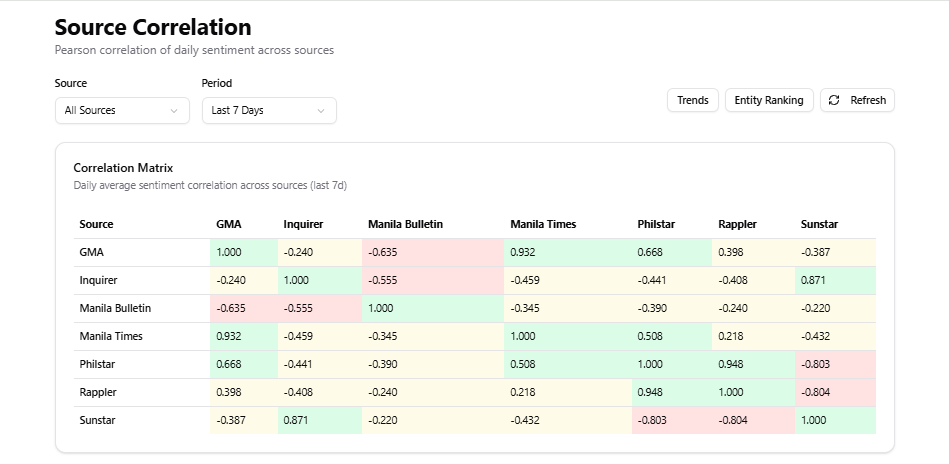
\includegraphics[width=\linewidth]{source-correlation-heatmap.png}}
  \caption{Cross-source sentiment correlation heatmap (Pearson $r$) based on daily average sentiment scores (March~25--31, 2026).}
  \label{fig:correlation-heatmap}
\end{figure}

The resulting matrix reveals several strong and contrasting relationships. Manila Bulletin shows a strong positive correlation with Philstar ($r=0.657$) and ABS-CBN ($r=0.687$), indicating that these outlets exhibit synchronized sentiment fluctuations over time. This suggests that they may be responding similarly to shared national events or dominant news narratives during the observation window.

In contrast, a strong negative correlation is observed between GMA and Manila Bulletin ($r=-0.668$), indicating opposing sentiment behavior across the same time period. Similarly, ABS-CBN and Manila Times exhibit a negative relationship ($r=-0.594$), reflecting divergence in sentiment direction.

Moderate positive correlations are observed between ABS-CBN and Inquirer ($r=0.621$), while weak or near-zero correlations (e.g., ABS-CBN and Philstar, $r=0.032$) suggest minimal linear association.

\begin{figure}[h]
  \centering
  \begin{subfigure}{0.49\linewidth}
    \centering
    \imgbox{\includegraphics[width=\linewidth]{GMA_new.png}}
    \caption{GMA daily average sentiment.}
    \label{fig:gma-new}
  \end{subfigure}
  \hfill
  \begin{subfigure}{0.49\linewidth}
    \centering
    \imgbox{\includegraphics[width=\linewidth]{MB_new.png}}
    \caption{Manila Bulletin daily average sentiment.}
    \label{fig:mb-new}
  \end{subfigure}
  \caption{Outlet-level sentiment trends for selected sources.}
  \label{fig:correlation-outlets}
\end{figure}

\textbf{GMA daily average sentiment.}
\begin{table}[h]
  \centering
  \small
  \begin{tabular}{lr}
    \toprule
    Date & GMA Hybrid score \\
    \midrule
    March 25 & -0.135 \\
    March 26 & -0.187 \\
    March 27 & -0.220 \\
    March 28 & -0.189 \\
    March 29 & -0.194 \\
    March 30 & -0.135 \\
    March 31 & -0.440 \\
    \bottomrule
  \end{tabular}
\end{table}

\textbf{Manila Bulletin daily average sentiment.}
\begin{table}[h]
  \centering
  \small
  \begin{tabular}{lr}
    \toprule
    Date & MB Hybrid score \\
    \midrule
    March 25 & -0.250 \\
    March 26 & -0.108 \\
    March 27 & -0.068 \\
    March 28 & 0.004 \\
    March 29 & 0.120 \\
    March 30 & -0.406 \\
    March 31 & 0.130 \\
    \bottomrule
  \end{tabular}
\end{table}

\textbf{Relationship between GMA and Manila Bulletin.}
Figure~\ref{fig:correlation-heatmap} shows a strong negative correlation between GMA and Manila Bulletin ($r=-0.668$). This indicates that the sentiment trends of the two outlets frequently move in opposite directions. As observed in Figure~\ref{fig:correlation-outlets}, Manila Bulletin gradually transitions into positive sentiment toward the latter part of the observation window, while GMA remains consistently negative, culminating in a sharp drop on March~31. This divergence in sentiment movement explains the strong inverse relationship captured by the Pearson coefficient.

\textbf{Sample Pearson calculation.}
To validate the computed correlations, a sample calculation was performed for GMA and Manila Bulletin using their daily average sentiment scores. Substituting the observed values into Equation~\ref{eq:pearson} yields a correlation coefficient of $r = -0.668$, matching the value obtained from the correlation matrix.

\textbf{Interpretation of cross-source relationships.}
These findings demonstrate that sentiment alignment across news sources is not uniform, but instead varies depending on editorial focus, topic selection, and framing. As a result, correlation patterns may serve as a proxy for detecting convergence or divergence in media narratives over time. Strong positive correlations suggest synchronized responses to shared events, while negative correlations indicate contrasting narrative tones or differing emphases across outlets.

\textbf{Note.}
Correlation values reflect statistical association only and do not imply causation or editorial influence. Sentiment scores in this study are derived from a hybrid approach combining a fine-tuned DistilBERT model and a modified VADER lexicon adapted for local linguistic context. While this approach improves robustness across both formal English and code-switched or localized expressions, limitations remain in handling sarcasm, implicit tone, and context-dependent meanings. These factors may introduce minor variations in sentiment estimation and should be considered when interpreting correlation results.

Overall, the analysis highlights the presence of both aligned and opposing sentiment clusters across Philippine news media. This suggests that while some outlets respond similarly to national events, others exhibit distinct tonal patterns, reflecting diversity in reporting perspectives.


\subsection{Most Frequent Entities and Their Sentiment Profiles}

This subsection summarizes entity frequency and the average sentiment associated with each entity’s coverage within the observation window. Named Entity Recognition (NER) was applied to extract PERSON, ORG, and GPE entities, which were then ranked by mention frequency and paired with their corresponding average sentiment scores.

\begin{figure}[h]
  \centering
  \imgbox{\maybeincludegraphics[width=\linewidth]{entities_chart.png}}
  \caption{Top mentioned entities with average sentiment scores.}
  \label{fig:entities}
\end{figure}

The results from Figure~\ref{fig:entities} indicate a strong dominance of institutional and political entities in the dataset. The most frequently mentioned entity is the Philippine National Police, with 638 mentions and an average sentiment score of $-0.533$, reflecting sustained negative or critical reporting. High-ranking political figures such as Rodrigo Duterte ($-0.439$), Ferdinand Marcos Jr. ($-0.469$), and Sara Duterte ($-0.465$) also appear prominently, suggesting that the news cycle is heavily centered on governance and political developments.

Institutional entities including the Senate ($-0.666$), Malacañang Palace ($-0.614$), and the Supreme Court ($-0.661$) further reinforce this trend, all exhibiting consistently negative sentiment. This pattern indicates that media coverage during the observation window is largely focused on legal proceedings, policy debates, and political tensions.

In contrast, geographic entities such as Manila ($-0.071$) and the Philippines ($-0.008$) exhibit near-neutral sentiment, reflecting their use as contextual references rather than subjects of evaluative reporting. International entities such as the United States ($-0.322$) and the Middle East ($-0.411$) show moderately negative sentiment, likely influenced by geopolitical tensions and conflict-related reporting.

\textbf{Contextual interpretation of top entities.}
To better understand why the top-ranked entities exhibit predominantly negative sentiment scores, a qualitative review of representative news articles was conducted. The findings suggest that the observed sentiment patterns are largely driven by the nature of reported events rather than inherent bias in the sources.

For instance, the Philippine National Police is frequently associated with crime-related reporting, including ambushes, killings, and large-scale security deployments. Articles describing such incidents naturally contain negative language (e.g., `killed,'' `attack,'' ``ambush''), contributing to its overall negative sentiment score.

This suggests that sentiment aggregation in news media is structurally skewed toward negativity, as high-frequency entities are disproportionately associated with conflict-driven events. Consequently, aggregate sentiment may reflect event selection bias rather than purely editorial tone, where the prominence of negative events leads to an overrepresentation of negative sentiment in system-level analysis.


Similarly, political figures such as Rodrigo Duterte, Sara Duterte, and Ferdinand Marcos Jr. are often mentioned in the context of legal proceedings, investigations, and political conflict. Coverage related to impeachment processes, International Criminal Court (ICC) cases, and governance issues tends to emphasize controversy and accountability, which are typically framed in negative terms.

Institutional entities such as the Senate and the Supreme Court are commonly referenced in reports involving legislative disputes, judicial reviews, and policy deliberations. These topics frequently involve disagreement, legal challenges, or crisis response, further contributing to negative sentiment aggregation.

International entities such as the Middle East and the United States also exhibit negative sentiment due to their association with geopolitical tensions, security concerns, and economic issues. News reporting in these contexts often emphasizes conflict, diplomacy, or instability, which inherently carries negative connotations.

These observations indicate that the dominance of negative sentiment among top entities is primarily a reflection of event-driven reporting patterns. News media tend to prioritize issues involving conflict, crisis, and accountability, resulting in a higher concentration of negative sentiment in aggregated analyses.

\textbf{Implication.}
This highlights an important limitation in sentiment-based media analysis: high-frequency entities associated with critical or conflict-driven events may appear disproportionately negative, not due to editorial bias, but due to the intrinsic nature of the events being reported. Therefore, sentiment scores should be interpreted alongside contextual analysis to avoid misleading conclusions regarding media tone or bias.

\textbf{Note.}
Minor entity classification noise (e.g., misclassification of non-person terms) may occur due to limitations of the NER model, but such cases were minimal and do not significantly affect the overall trends observed.

\section{Conclusion}
This study designed and implemented PH VibeCheck AI, an automated media monitoring system for Philippine online news. The platform integrates scheduled web scraping, text normalization, hybrid sentiment analysis (Tagalog/Taglish-extended VADER combined with DistilBERT), and named entity extraction, and presents results through interactive analytics for trend monitoring and cross-source comparison.

The system continuously collects and processes articles from multiple outlets, persisting normalized article records, sentiment outputs, and scraping logs in a relational database to support traceability and reproducible aggregation. Quantitative results reported in this paper are based on a fixed observation window (March~25--March~31, 2026), with data collected and processed as of April~1, 2026. This window was selected to ensure complete daily coverage across all sources and to minimize inconsistencies due to missing or partial data.

PH VibeCheck AI supports sentiment trend summaries, cross-source correlation analysis, and entity-level aggregation, illustrating how statistical summaries and NLP outputs can be combined to surface patterns in large-scale news streams. These outputs are intended as exploratory indicators to guide deeper qualitative review rather than definitive judgments about intent or bias.

\subsection{Limitations}
This study is subject to several limitations. First, the hybrid sentiment engine remains sensitive to domain mismatch: DistilBERT is trained on general sentiment data and may misinterpret news-specific framing, while the Tagalog/Taglish VADER patch is incomplete and may not capture emerging slang or domain-specific polarity shifts. Additionally, both models may struggle with sarcasm, implicit tone, and culturally nuanced expressions, particularly in code-switched or localized language.

Second, the hybrid routing mechanism relies on heuristic language signals and may misroute highly mixed-language articles. News sources may also publish content in languages beyond English and Tagalog (e.g., Cebuano), which can introduce noise into sentiment estimation. Minor inaccuracies may also arise from Named Entity Recognition (NER), particularly for ambiguous or context-dependent terms.

Third, the reliance on online news articles introduces inherent selection bias. Media coverage tends to prioritize conflict, crisis, and high-impact events, which may lead to a systematic skew toward negative sentiment in aggregated results. As a result, observed sentiment patterns may reflect the distribution of reported events rather than purely editorial tone.

Finally, the correlation analysis is limited to linear relationships and does not capture more complex temporal or causal dynamics between sources. In addition, scraper downtime and website layout changes may result in missing data and uneven source coverage within the observation window.

\subsection{Recommendations}
\begin{itemize}
    \item \textbf{Transition to Multilingual Transformers:} Replace the binary DistilBERT model with a stronger multilingual architecture, such as \textit{XLM-RoBERTa} or \textit{Tagalog-RoBERTa}. These models are pre-trained on diverse linguistic corpora, significantly improving the classification of code-switched (Taglish) news and reducing the false-polarization of neutral factual reporting.
    
    \item \textbf{Expansion of the Tagalog/Taglish Lexicon:} Supplement the VADER+PH patch with a broader dictionary of localized affective terms, including colloquialisms (\textit{hugot, lodi, budol}) and political jargon (\textit{aspeto, mambabatas, krisis}), to ensure the rule-based component captures nuance that pure transformers might miss in short-form headlines.
    
    \item \textbf{Gold-Standard Dataset Construction:} Develop a manually annotated ``Gold Set'' of Philippine news sentiment (n > 1,000) to move beyond lightweight manual benchmarks. This enables objective calculation of Precision-Recall curves and supports more defensible, peer-reviewed performance reporting.
    
    \item \textbf{Advanced Entity Disambiguation:} Implement Named Entity Recognition (NER) specifically tuned for Philippine contexts to resolve ambiguities between local figures, acronyms (e.g., distinguishing between \textit{BSP} as the central bank vs. Boy Scouts), and geopolitical variants.
    
    \item \textbf{Automated Data Quality Monitoring:} Deploy real-time observability tools to audit scraper health. This should include automated detection of "silent failures" like empty datelines, repeated boilerplate text, or source-specific structural changes that degrade dataset integrity.
    
    \item \textbf{Dynamic Temporal Analysis:} Enhance the platform's filtering logic to support arbitrary date-range queries. This allows researchers to perform comparative sentiment studies across specific historical events, such as election cycles or national emergencies, rather than relying on fixed 7-day windows.
\end{itemize}

\subsection{Artifact / Source Code Availability}
To support reproducibility, the PH VibeCheck AI source code and evaluation scripts are publicly available on GitHub \cite{pheye_github}. The repository includes build/run instructions and a pinned version corresponding to the system configuration used for the reported snapshot. Due to copyright and licensing constraints of publisher content, the study does not redistribute full article text; instead, it provides the software pipeline, database schemas, and aggregated outputs necessary to replicate the analysis on newly collected data.

\begin{acks}
The author thanks Dr.\ Lea P.\ Ymalay and Guimaras State University for guidance and support during this capstone project.
\end{acks}

\bibliographystyle{ACM-Reference-Format}
\bibliography{references}

\end{document}
